In the last chapter, we introduced new language facilities that can be used by
the programmer to coordinate execution. This new approach retains the implicit
parallelism of the standard LM language but it does not allow the programmer to
fully reason about the underlying parallel architecture. The only architecture
reasoning allowed relates to node partitioning and movement between threads. In
principle, it should be advantageous to reason about thread state, that is, to
perform rule inference about facts stored on each thread and allow threads to
communicate and coordinate between them depending on their current state. This
would introduce a kind of explicit parallelism into an implicitly parallel
language such as LM. However, this explicit parallelism remains declarative
since it should remain easy to prove properties about the thread's state.

\section{Rationale: Graph Searching}
Consider the problem of checking if a set of nodes $S$ in a graph $G$ is
reachable from an arbitrary node $N$. An obvious solution to this problem is to
start at $N$, gather all the neighbor nodes into a list and then recursively
visit all those reachable nodes, until $S$ is covered. This reduces to a problem
of performing a breadth or depth-first search on graph $G$. However, this
solution is sequential and does not have much concurrency.  An alternative
solution to the problem is to recursively propagate the search to all neighbors
and aggregate the results in the node where the search started.  The code for
this later solution is shown in Fig.~\ref{code:threads:reach_simple}.

\begin{figure}[h]
\begin{Verbatim}[numbers=left,fontsize=\codesize,commandchars=*\#\&]
type int id.*hfill// Type declaration
type list int reach-list.

type edge(node, node).*hfill// Predicate declaration
type value(node, int).
type linear search(node, id, reach-list).
type linear do-search(node, id, node, reach-list).
type linear lookup(node, id, reach-list, int Val).
type linear new-lookup(node, id, int Val).
type linear visited(node, id).

search(A, Id, ToReach)*label#line:threads:reach_lookup1&*hfill// Rule 1: initialize search
   -o do-search(A, Id, A, ToReach),
      lookup(A, Id, ToReach, []).*label#line:threads:reach_lookup2&

lookup(A, Id, ToReach, Found), new-lookup(A, Id, Val)*hfill// Rule 2: new reachable node found
   -o lookup(A, Id, remove(ToReach, Val), [Val | Found]).

do-search(A, Id, Node, ToReach),*label#line:threads:reach_visit1&*hfill// Rule 3: node has already seen this search
visited(A, Id)
   -o visited(A, Id). *label#line:threads:reach_visit2&

do-search(A, Id, Node, ToReach),*hfill// Rule 4: node found and propagate search
!value(A, Val), Val in ToReach*hfill// New node was found.
   -o visited(A, Id),*label#line:threads:reach_visit_visited1&
      new-lookup(Node, Id, Val),
      {B | !edge(A, B) -o do-search(B, Id, Node, remove(ToReach, Val))}.*label#line:threads:reach_propagate&

do-search(A, Id, Node, ToReach),*hfill// Rule 5: node not found and propagate search
!value(A, Val), ~ Val in ToReach*hfill// Not the node we are looking for.
   -o {B | !edge(A, B) -o do-search(B, ID, Node, ToReach)},*label#line:threads:reach_propagate2&
      visited(A, Id).*label#line:threads:reach_visit_visited2&
\end{Verbatim}

\caption{LM code to perform reachability checking on a graph.}
\label{code:threads:reach_simple}
\end{figure}

Each distinct reachability search is represented by a number (\code{Id}) and a
\code{search} axiom. Associated to each search \code{Id} is a list of nodes to
reach.  The predicate \code{visited} marks nodes that have already
participated in search, while predicate \code{do-search} is used to propagate a
specific search. The first rule
(lines~\ref{line:threads:reach_lookup1}-\ref{line:threads:reach_lookup2}) starts
a particular search by deriving a \code{do-search} and an \code{lookup} fact.
The \code{lookup} fact is used as an accumulator and is stored in the starting
node. The third rule
(lines~\ref{line:threads:reach_visit1}-\ref{line:threads:reach_visit2}) avoids
visiting the same node twice in the presence of a \code{visited} fact.  This
visited fact is derived in the next two rules
(lines~\ref{line:threads:reach_visit_visited1}
and~\ref{line:threads:reach_visit_visited2}).  If the node where the search is
being performed is in the set of nodes we want to reach (\code{ToReach}) then we
remove the node value from the list and propagate the search to the neighbor
nodes (line~\ref{line:threads:reach_propagate}).  Otherwise, the search is
propagated but no value is removed from \code{ToReach}.

As an example, consider Fig.~\ref{fig:threads:reach_example}, which shows 2
reachability checks on a graph with 10 nodes. For instance, the search with
\code{Id = 0} starts at node \code{@1} and checks if nodes \code{@1}, \code{@2},
and \code{@3} are reachable from \code{@1}. Since \code{@1} is the starting
node, \code{1} is immediately removed from the reachable list, including the
propagated \code{do-search} facts but also the \code{lookup} fact that is stored
at node \code{@1}. Once \code{do-search} reaches node \code{@3}, the value
\code{3} is removed from the list and a new \code{do-search} is propagated to
node \code{@1} (not shown in the figure) and \code{@2}. At the same time, node
\code{@2} receives the list \code{[2,3]}, removes \code{2} and propagates
\code{[3]} to node \code{@3} and \code{@1}. Node \code{@1} receives two
\code{new-lookup} facts, one from \code{@3} and another from \code{@2}, due to
successful searches and the \code{lookup} fact becomes \code{lookup(@1,0,[],
[1,2,3])}.

The attentive reader will notice that node \code{@1} already knows that all the
nodes have been reached and that nodes \code{@7} and \code{@4} will, needlessly,
continue to check if \code{[2,3]} are reachable. This is an issue that arises
because the programmer has valued concurrency by increasing redundancy and
reducing communication between nodes. It would be prohibitly expensive to share
reachability information between nodes. An alternative solution is to store the
results of the search on the thread performing the search and then coordinate
the results with other threads since the number of threads is usually smaller
than the number of nodes. Before showing how the reachability program is solved
using thread-based facts, we first present the changes to the language.

\begin{figure}[ht]
\begin{center}
   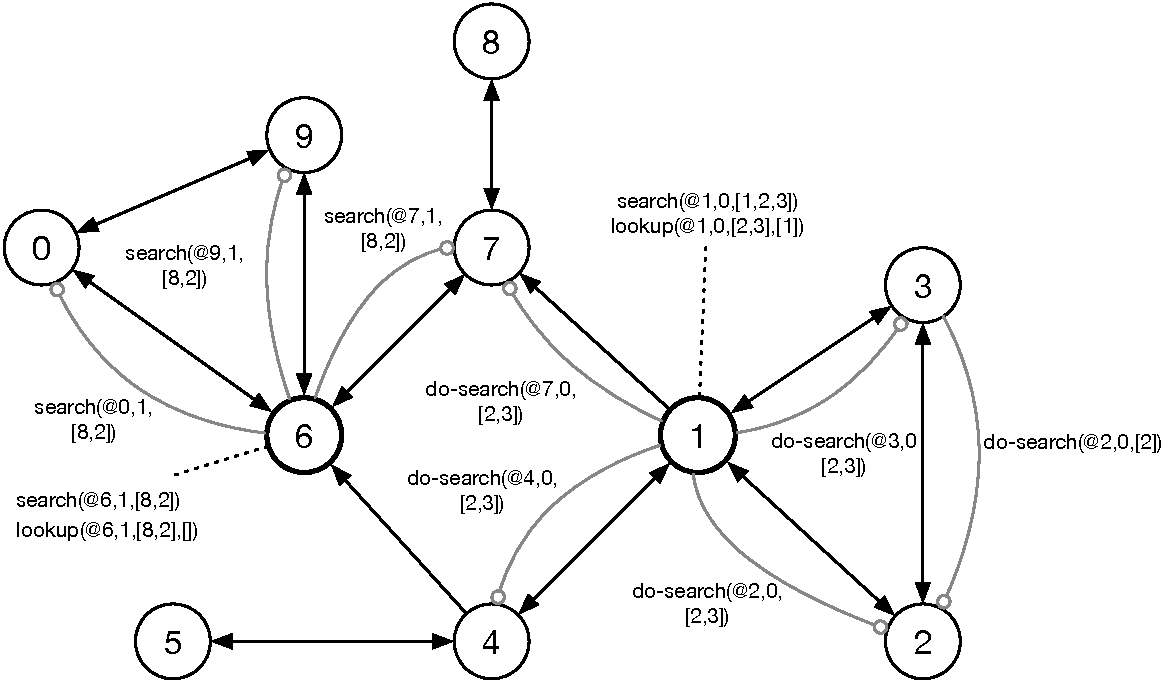
\includegraphics[width=0.9\linewidth]{figures/threads/reach.pdf}
\end{center}

\caption{Performing reachability checks on a graph using nodes \code{@1}
(\code{Id = 0}) and \code{@6} (\code{Id = 1}).  Search with \code{Id = 0} wants
to reach nodes \code{@1}, \code{@2}, and \code{@3} from node \code{@1}. Since
\code{@1} is part of the target nodes, the fact \code{do-search} propagated to
neighbor nodes does not include \code{1}.}

\label{fig:threads:reach_example}
\end{figure}

\subsection{Language Changes}

In the previous chapter, we presented coordination facts such as
\code{thread-id} and \code{set-thread} that already bring some awareness about
the underlying parallel system. Furthermore, such facts also introduce the
\code{thread} type for predicate arguments, which refers to a thread in the
system that is related to a core in a multi core processor. We now introduce the
concept of \emph{thread facts}, which are logical facts stored at the thread
level, meaning that, each thread is now an entity with its own logical facts.
The type \code{thread} is also now the type of the first argument of
\emph{thread predicates}, indicating that the predicate is related and is to be
stored in a specific thread. We also view the available threads as forming a
separate graph from the data graph, a graph of the processing units which are
operating on the data graph.

The introduction of thread facts increases the expressiveness of the system in
the sense that it is now possible to write inference rules that reason about the
state of the threads. This creates optimization opportunies since we can now
write algorithms with global information stored in the thread, while keeping the
LM language fully declarative. Moreover, threads are now allowed to explicitly
communicate with each other, and in conjunction with coordination predicates,
enable the writing of complex scheduling policies.

We discriminate between two new types of inference rules. The first type is the
\emph{thread rule} and has the form \code{a(T), b(T) -o c(T)}, and can be read
as: if thread \code{T} has fact \code{a(T)} and \code{b(T)} then derive fact
\code{c(T)}. The second type is the \emph{mixed rule} and has the form
\code{a(T), d(N) -o e(N)} and can be read as: if thread \code{T} is executing
node \code{N} and has the fact \code{a(T)} and node \code{N} has the fact
\code{d(N)} then derive \code{e(N)} at node \code{N}. Thread rules reason solely
at the thread level, while mixed rules allow reasoning about both thread and
node facts. Logically, the mixed rule uses an extra fact \code{running(T, N)},
which indicates that thread \code{T} is currently executing node \code{N}. The
\code{running} fact is implicitly retracted and asserted every time the thread
selects a different node for execution. This makes our implementation efficient
since a thread does not need to look for nodes that match mixed rules and it is
then the scheduling of the program that drives the matching of such rules.

\subsection{Graph Of Threads}

Figure~\ref{fig:coord:thread_facts} represents a schematic view of the two graph
data structures of a program with three threads: thread $T1$ is executing node
\code{@5}, $T2$ is executing node \code{@4}, and $T3$ is executing node
\code{@3}. Note that every thread has access to its own facts and to the node
facts.

\begin{figure}[ht]
   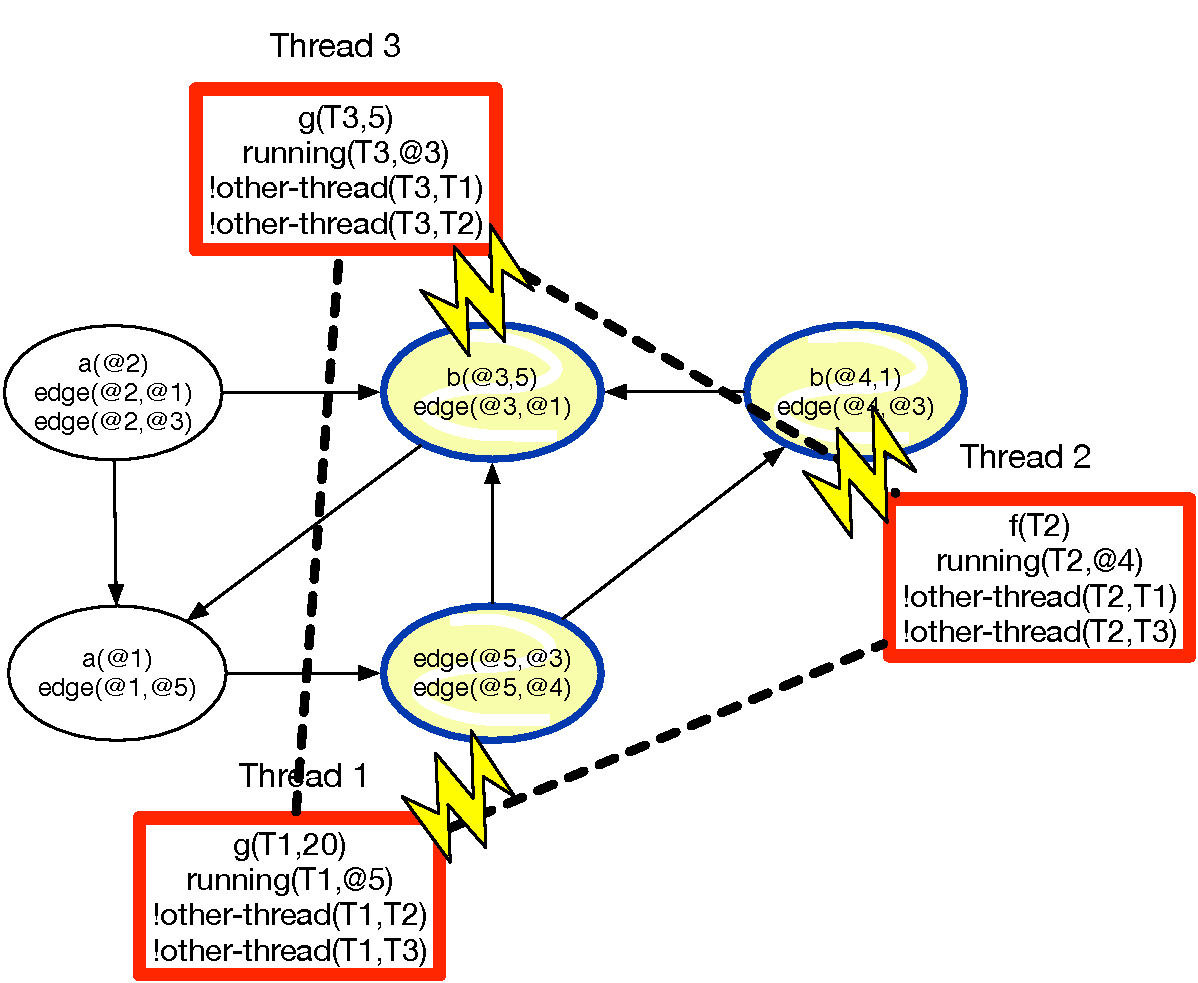
\includegraphics[width=0.6\linewidth]{figures/threads/threads.pdf}

   \caption{An example program being executed with three threads. Note that each
      threads has a \code{running} fact that stores the node currently being
   executed.}

   \label{fig:coord:thread_facts}
\end{figure}

We added several helpful predicates that allow the programmer to inspect the
graph of threads and reason about the state of computation as it relates to
threads:

\begin{itemize}
   \item \code{\bang thread-list(T, L)}: Fact instantiated in all threads where
      \code{L} is a list of all threads executing in the system.

   \item \code{\bang other-thread(T1, T2)}: Connects thread \code{T1} to all the
      other threads \code{T2} executing in the system. Note that in
      Fig.~\ref{fig:coord:thread_facts}, we use \code{\bang other-thread} fact
      to specify the graph of threads.


   \item \code{\bang leader-thread(T, TLeader)}: Fact instantiated in all
      threads where \code{TLeader} refers to a selected thread (the first thread
      in \code{L} of \code{\bang thread-list(T, L)}).

   \item \code{running(T, A)}: Used to retrieve the current node \code{A}
      running on thread \code{T}.
\end{itemize}

With the exception of \code{running}, every other fact is added at the beginning
of the program as a persistent fact.

\subsection{Reachability With Thread Facts}

We know update the graph reachability program presented in
Fig.~\ref{code:threads:reach_simple} to use thread facts in order to avoid
needless searches on the graph. The search process is still done concurrently as
before, but the search state is now stored in each thread, allowing the thread
to store partial results and coordinate with other threads. The code for this new
version is shown in Fig.~\ref{code:threads:reach_threads}.

Lines~\ref{line:threads:reacht_start1}-\ref{line:threads:reacht_start2} start
the search process by assigning a thread \code{Owner} to search \code{Id} using
the persistent fact \code{\bang thread-list} which contains the list of all
available threads in the system. Next, in
line~\ref{line:threads:reacht_threads}, a fact \code{thread-search} is created
for all threads using a comprehension. We use predicate \code{do-search} to
propagate the search through the graph and a predicate \code{visited} to mark
nodes already processed for a specific search.  The two rules in
lines~\ref{line:threads:reacht_check1}-\ref{line:threads:reacht_check2}
propagate the search process to the neighbor nodes and check if the current node
is part of the list of nodes we want to reach.

An interesting property of this version is that each owner thread responsible
for a search keeps track of the remaining nodes that need to be reached. In
line~\ref{line:threads:reacht_remove}, we derive \code{remove-thread-search} in
order to inform owner threads about new reachable nodes. Once an owner thread
detects that all nodes have been reached (lines
\ref{line:threads:reacht_reached1}-\ref{line:threads:reacht_reached2}), all the
other threads will know that and update their search state accordingly
(lines~\ref{line:threads:reacht_knows1}-\ref{line:threads:reacht_knows2}). When
every thread knows that all nodes were reached, they will consume
\code{do-search} facts (lines
\ref{line:threads:reacht_prune1}-\ref{line:threads:reacht_prune2}), effectively
pruning the search space.

\begin{figure}[h]
\begin{Verbatim}[numbers=left,fontsize=\codesize,commandchars=*\#\&]
search(A, Id, ToReach),*label#line:threads:reacht_start1&*hfill// Rule 1: initialize search
*textbf#!thread-list(T, L)&, Owner = nth(L, Id % @threads)*hfill// Allocate search to a thread
   -o {T2 | *textbf#!other-thread(T, T2)& -o *textbf#thread-search(T2, Id, ToReach, Owner)&},*label#line:threads:reacht_threads&
      do-search(A, Id).*label#line:threads:reacht_start2&

*textbf#thread-search(T, Id, [], Owner)&, *label#line:threads:reacht_prune1&*hfill// Rule 2: search completed
do-search(A, Id)
   -o *textbf#thread-search(T, Id, [], Owner)&. *label#line:threads:reacht_prune2&

do-search(A, Id),*hfill// Rule 3: node already visited
visited(A, Id)
   -o visited(A, Id).

do-search(A, Id),*label#line:threads:reacht_check1&*label#line:bfs_join1&*hfill// Rule 4: node found
*textbf#thread-search(T, Id, ToReach, Owner)&,*label#line:threads:reacht_join2&
!value(A, Val), Val in ToReach
   -o *textbf#thread-search(T, Id, remove(ToReach, Val), Owner)&,
      *textbf#remove-thread-search(Owner, Id, Val)&,*hfill// Tell owner thread about it.*label#line:threads:reacht_remove&
      {B | !edge(A, B) -o do-search(B, Id)},
      visited(A, Id).

do-search(A, Id),*hfill// Rule 5: node not found but propagate search
*textbf#thread-search(T, Id, ToReach, Owner)&,
!value(A, Val), ~ Val in ToReach
   -o *textbf#thread-search(T, Id, ToReach, Owner)&,
      visited(A, Id),
      {B | !edge(A, B) -o do-search(B, Id)}.*label#line:threads:reacht_check2&

*textbf#remove-thread-search(T, Id, Val), thread-search(T, Id, ToReach, Owner)&*hfill// Rule 6: node found
   *textbf#-o thread-search(T, Id, remove(ToReach, Val), Owner),&
      *textbf#check-results(T, Id).&

*textbf#check-results(T, Id),&*label#line:threads:reacht_reached1&*hfill// Rule 7: search is completed
*textbf#thread-search(T, Id, [], Owner)&
   *textbf#-o thread-search(A, Id, [], Owner),&
      *textbf#{B | !other-thread(T, B) -o signal-thread(B, Id)}.&*label#line:threads:reacht_reached2&

 *textbf#check-results(T, Id),&*hfill// Rule 8: search not completed yet
 *textbf#thread-search(T, Id, ToReach, Owner), ToReach <> []&
   *textbf#-o thread-search(T, Id, ToReach, Owner).&

*textbf#signal-thread(T, Id),&*hfill// Rule 9: thread knows search is done*label#line:threads:reacht_knows1&
*textbf#thread-search(T, Id, ToReach, Owner)&
   *textbf#-o thread-search(T, Id, [], Owner).& *label#line:threads:reacht_knows2&
\end{Verbatim}
\caption{Coordinated version of the reachability checking program. Note
that \code{@threads} represent the number of threads in the system.}
\label{code:threads:reach_threads}
\end{figure}

An alternative implementation could force every thread to share its reached
nodes to all the other threads in the system. However, this would generate a lot
of traffic between threads, which would actually make the program perform worse.
Our final solution is a good trade off since it only forces threads to
coordinate when pruning can actually happen.

Figure~\ref{fig:threads:results_search} presents experimental results of the
graph reachability program using 4 different datasets. Except for Random, all
the datasets were already used in the MSSD program and were presented before.
The Random dataset is a randomly generated graph with 50000 nodes and about a
million edges.  In the plots, we show the run time of the version without thread
facts (\textbf{Regular}) and the version using thread facts called
\textbf{Threads}. We also show the speedup of the \textbf{Threads} and
\textbf{Regular} versions against the \textbf{Regular} version with 1 thread.

Our results indicate that using thread facts produces a significant reduction in
run time. This is especially true in the case of datasets with large number of
edges, since less facts are produced and propagated in the graph when the
threads know that the search has been completed. The results also show that, in
the case of the Facebook dataset, in which the number of queries is the same as
the number of nodes, the use of thread facts does not produce great improvements
due to the costs of managing the reachability results on each thread's database.
These costs are related to the need to index and lookup \code{thread-search}
facts on the \code{Id} argument every time a node is inspected.

\begin{figure}[]
        \centering
        \begin{subfigure}[b]{\plotsize\textwidth}
           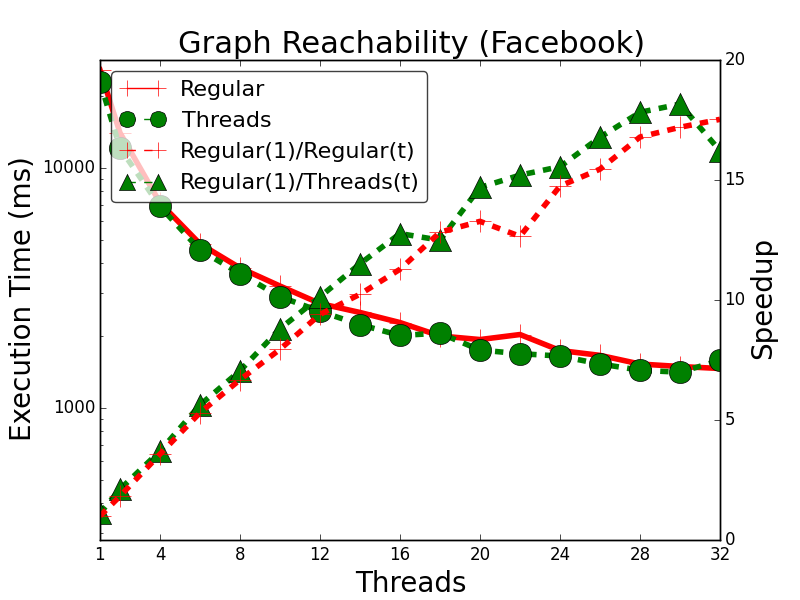
\includegraphics[width=\textwidth]{experiments/threads/cmp-search-facebook.png}
           \caption{Facebook has 2000 nodes and 20000 edges. The dataset makes
           2000 graph queries to 5\% of the graph's nodes.}
           \label{fig:threads:search_facebook}
        \end{subfigure}
        \spacing
        \begin{subfigure}[b]{\plotsize\textwidth}
           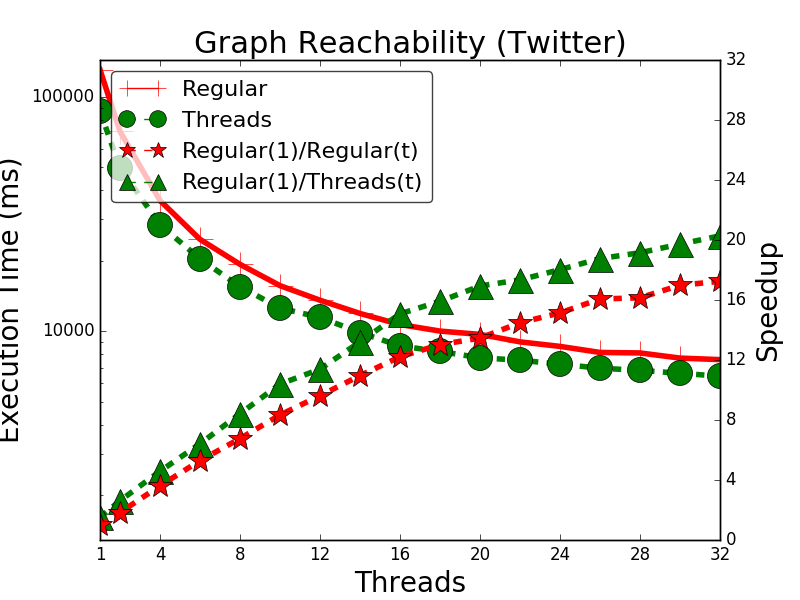
\includegraphics[width=\textwidth]{experiments/threads/cmp-search-twitter.png}
           \caption{Twitter has 81306 nodes and 1768149 edges. The dataset makes
           100 graph queries to 1\% of the graph's nodes.}
           \label{fig:threads:search_twitter}
        \end{subfigure} \\
        \begin{subfigure}[b]{\plotsize\textwidth}
           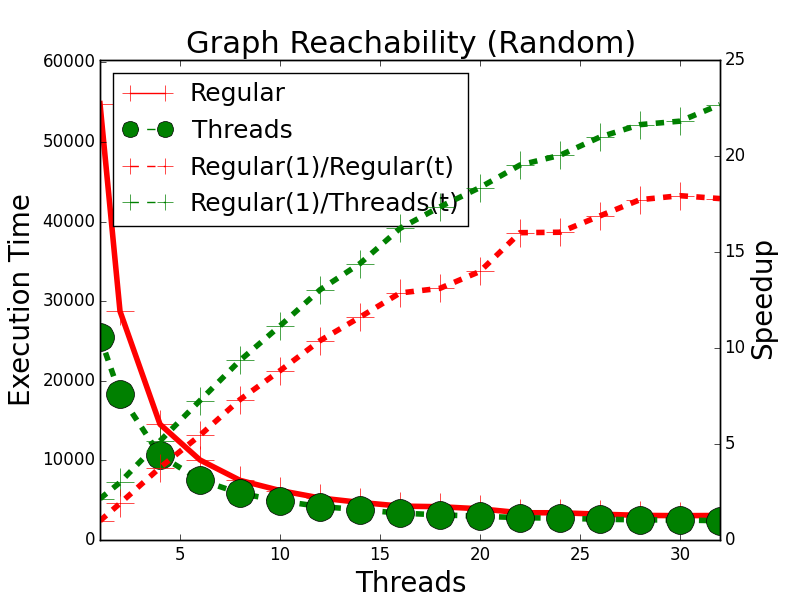
\includegraphics[width=\textwidth]{experiments/threads/cmp-search-random.png}
           \caption{Random is a graph with 50000 nodes and 1052674
              edges. The dataset makes 20 graph queries
              to 5\% of the graph's nodes.}
           \label{fig:threads:search_random}
        \end{subfigure}
        \spacing
        \begin{subfigure}[b]{\plotsize\textwidth}
           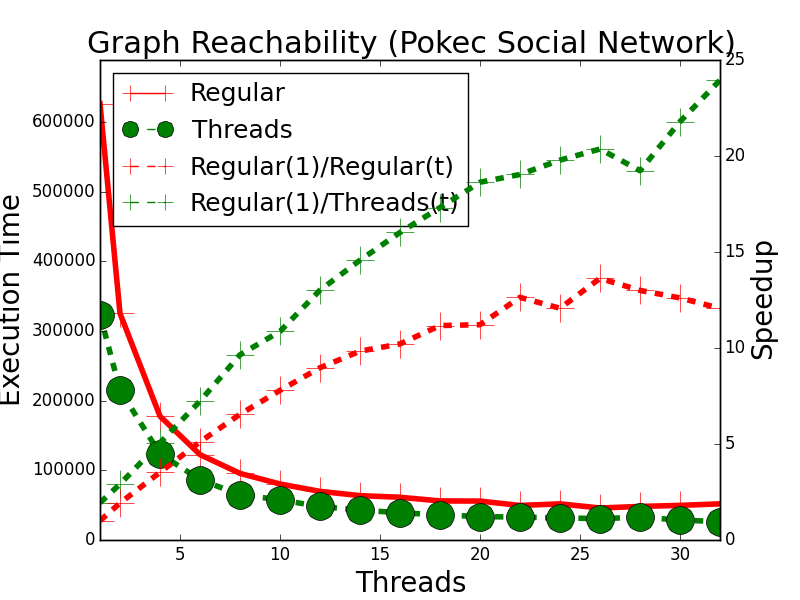
\includegraphics[width=\textwidth]{experiments/threads/cmp-search-pokec.png}
           \caption{Pokec has 1632803 nodes and 30622564 edges. The dataset
           makes 3 graph queries to 1\% of the graph's nodes.}
           \label{fig:threads:search_pokec}
        \end{subfigure} \\
        \caption{Measuring the performance of the graph reachability program
        when using thread facts.}
        \label{fig:threads:results_search}
\end{figure}

The graph reachability program shows how to introduce complex coordination
policies between threads by reasoning about the state of each thread. In
addition, the use of linear logic programming makes it easier to prove
properties of the program since computation is done by applying controlled
changes to the state.


\clearpage


\section{Implementation Changes}
The compilation and runtime system described in
Chapter~\ref{chapter:implementation} requires ysome changes in both the compiler
and in the runtime system to support thread-based facts.

\subsection{Compiler}

The compiler needs to recognize rules that use thread facts. For thread rules,
the compiler checks if the rule's body is using facts from the same thread by
checking the first argument of each fact. For mixed rules, the rule's body may
use a thread \code{T} and a node \code{A} and all the node facts have to use
\code{A}, while all threads facts must use \code{T} as the first argument. If
the programmer was to retrieve either the thread or the node for the current
computation, she may use \code{running(T, A)}.

Once rules are type checked, the iteration code for thread-based facts
needs to change. The database iterator will refer to the current thread in order to
fetch candidate facts since using the standard node database will return an
empty iterator. The runtime API used for inserting thread facts is also
different since they have to be added to the thread's database.

\subsection{Runtime}

Each thread has its own database of facts that is identical to a regular node
but only contains thread predicates. The major difference between a regular node
and a thread node is that a thread node is never put into the work queue of its
thread. As shown in the updated work loop presented in
Fig.~\ref{alg:threads:work_loop}, the thread node executes alongside the regular
node when $TH.process\_node$ is called. It is also important to note that,
before a thread becomes idle, it may have potential candidate thread rules that
are now derivable because another thread has derived thread facts in the current
thread. Note that it is entirely possible to have programs that only deal with
thread facts. These kinds of programs use only explicit parallelism.

\begin{figure}
\begin{algorithm}[H]
\KwData{Thread TH, THREADS}
\While{true}{
  $node \longleftarrow TH.work\_queue.pop\_node()$ \;
  \uIf{$node$}{
        \tcc{Have to use the thread's node}
        \underline{$TH.process\_node(node, TH.my\_node)$}\;
  }
  \Else{
     $target \longleftarrow random(len(THREADS))$\;
     $i \longleftarrow 0$\;
     \For{$i < len(THREADS)$}{
        $target \longleftarrow (target + 1) \% len(THREADS)$\;
        $nodes = THREADS[target].steal\_half()$\;
        \If{$len(nodes) > 0$}{                                                                                                    $TH.work\_queue.add\_to\_queue(nodes)$\;
           break\;
        }
        $i \longleftarrow i + 1$\;
     }
     \If{$len(TH.work\_queue) == 0$}{
        \tcc{The thread's node may have candidate rules using incoming thread facts}
        \underline{$TH.process\_node(nil, TH.my\_node)$}\;
        $TH.become\_idle()$\;
        \If{$TH.synchronize\_termination()$}{
           \Return{}\;
        }
        $TH.become\_active()$\;
     }
  }
}
\end{algorithm}
\caption{Thread work loop updated to take into account thread-based facts.
New and modified code is underlined.}
\label{alg:threads:work_loop}
\end{figure}

Thread facts also add points of synchronization the runtime system. For
instance, when a rule derives a new thread fact on another thread, it needs to
synchronize with that thread (using locks) to add the facts to the thread's
database.

\subsubsection{Matching Rules}

Matching rules using thread facts requires special care since some rules may
require both facts from a node and from a thread. Before a node is executed, the
matching engine of the regular node is updated to take into account the facts in
the thread. If the mixed rules are activated, they need to be executed, even if
they have failed under a different node. The reason is simple: the rule
constraints may now hold under the current node's database and therefore the
rule needs to be executed again.

\subsection{Graph Of Threads}

We added several helpful predicates that allow the programmer to inspect the
graph of threads and reason about the state of computation as it relates to
threads.

\begin{itemize}
   \item \code{\bang thread-list(T, L)}: Fact instantiated in all threads where
      \code{L} is a list of all threads executing in the system.

   \item \code{\bang other-thread(T1, T2)}: Connects thread \code{T1} to all the
      other threads \code{T2} executing in the system.

   \item \code{\bang leader-thread(T, TLeader)}: Fact instantiated in all
      threads where \code{TLeader} refers to a selected thread (usually the
      first thread in \code{L} of \code{\bang thread-list(T, L)}).

   \item \code{running(T, A)}: Used to retrieve the current node \code{A}
      running on thread \code{T}.
\end{itemize}

With the exception of \code{running}, every other fact is added at the beginning
of the program as a persistent axiom.


\section{Applications}

We present more applications that demonstrate the usefulness and power of thread-based facts.

\subsection{Binary Search Trees: Caching Results}
In Section~\ref{sec:language:key_value} we have presented an algorithm for
replacing a key's value in a BST dictionary. To make the program more
interesting, we consider a sequence of $n$ lookup or replace operations for
different keys in the BST (which may or may not be repeated). A single lookup or
replace has worst-case time complexity $\mathcal{O}(h)$ where $h$ is the height
of the BST, therefore performing $n$ operations takes $\mathcal{O}(h \times n)$
time.

In order to reduce the execution time of the new program, we can cache the
search and replace operations so that repeated operations become faster. Instead
of traversing the entire height of the BST, we look in the cache and send the
operation immediately to the node where the key is located. Without thread
facts, we might have cached the results at the root node, however, this is not a
scalable approach as it would introduce a serious bottleneck.

Figure~\ref{code:threads:btree_lookup_cache} shows the updated BST code with a thread
cache. We just added two more predicates, \code{cache} and
\code{cache-size}, that are facts placed in the thread and represent cached
keys and the total size of the cache, respectively. We also added three new
rules that handle the following cases:

\begin{enumerate}
      \item A key is found and is also in the cache
         (lines~\ref{line:threads:kv_rule1_start}-\ref{line:threads:kv_rule2_end})

      \item A key is found but is not in the cache
         (lines~\ref{line:threads:kv_rule2_start}-\ref{line:threads:kv_rule2_end});

      \item A key is in the cache, therefore a \code{replace} fact is
         derived in the target node
         (lines~\ref{line:threads:kv_rule3_start}-\ref{line:threads:kv_rule3_end}).

\end{enumerate}

Note that it is quite easy to extend the cache mechanism to use an LRU type
approach in order to limit the size of the cache.

\begin{figure}[ht]
\begin{Verbatim}[numbers=left,fontsize=\codesize,commandchars=*\{\}]
type left(node, node).
type right(node, node).
type linear value(node, int Key, string Value).
type linear replace(node, int Key, string Value).
type linear cache(thread, node, int).
type linear cache-size(thread, int).

// (1) Key exists and is also in the cache.*label{line:threads:kv_rule1_start}
replace(A, Key, RValue),
value(A, Key, Value),
*textbf{cache(T, A, Key)}
   -o value(A, Key, RValue).
      *textbf{cache(T, A, Key)}.*label{line:threads:kv_rule1_end}

// (2) Key exists and is not in the cache.*label{line:threads:kv_rule2_start}
replace(A, Key, RValue),
value(A, Key, Value),
*textbf{cache-size(T, Total)}
   -o value(A, Key, RValue),
      *textbf{cache-size(T, Total + 1)},
      *textbf{cache(T, A, Key)}.*label{line:threads:kv_rule2_end}

// (3) Cached by the thread.*label{line:threads:kv_rule3_start}
replace(A, RKey, RValue),
*textbf{cache(T, TargetNode, RKey)}
   -o replace(TargetNode, RKey, RValue),
      *textbf{cache(T, TargetNode, RKey)}.*label{line:threads:kv_rule3_end}

replace(A, RKey, RValue),
value(A, Key, Value),
!left(A, B),
RKey < Key
   -o value(A, Key, Value),
      replace(B, RKey, RValue). // go left

replace(A, RKey, RValue),
value(A, Key, Value),
!right(A, B),
RKey > Key
   -o value(A, Key, Value),
      replace(B, RKey, RValue). // go right
\end{Verbatim}
\caption{LM program for performing lookups in a BST with a thread cache.}
\label{code:threads:btree_lookup_cache}
\end{figure}


\subsection{PowerGrid Problem}
Consider a power grid with $C$ consumers and $G$ generators. We are interested
in connecting each consumer to a single generator, but each generator has a
limited capacity and the consumer draws a certain amount of power from the
generator. A valid power grid is built in such a way that all consumers are
serviced by a generator and that no generator is being overdrawn by too many
consumers. Although consumers and generators may be connected through a complex
network, we analyze the simple case where any consumer is able to attach to any
generator.

\begin{wrapfigure}{r}{0.5\textwidth}
   \begin{center}
      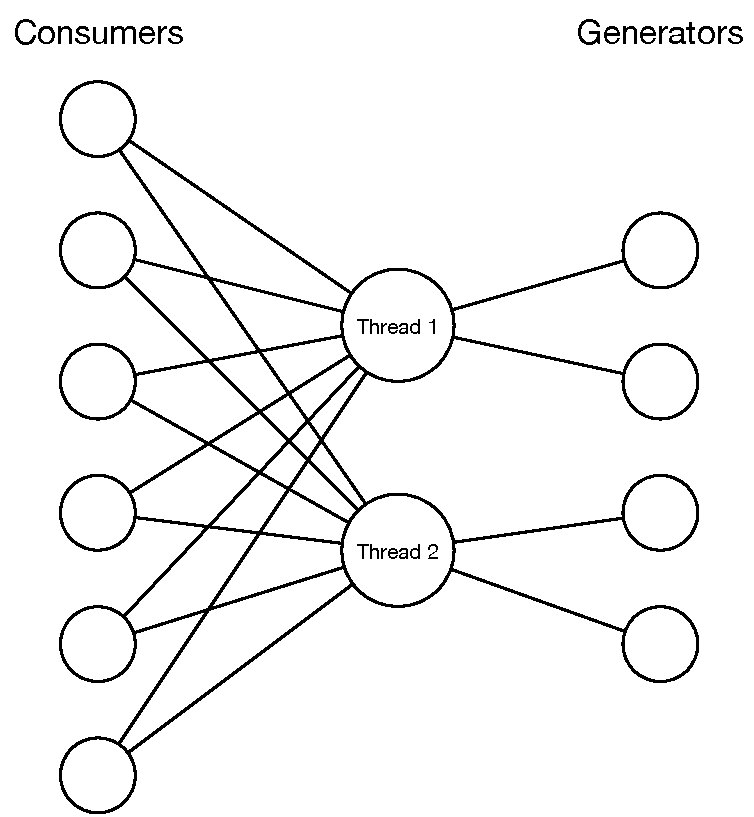
\includegraphics[width=1\linewidth]{figures/threads/powergrid.pdf}
   \end{center}
   \mycap{Configuration of a powergrid with 6 consumers, 4
      generators and 2 threads, with each thread responsible for 2 generators.}
   \label{fig:threads:powergrid}
\end{wrapfigure}

A straightforward distributed implementation for the PowerGrid problem requires
that each consumer is able to connect to any generator. Once a generator
receives a connection request, it may or may not accept it. If the generator has
no power available for the new consumer, it will disconnect from it and the
consumer must select another generator. This randomized algorithm works but may
take a long time to converge, depending on the amount of power available in the
generators. Figure~\ref{code:threads:powergrid} shows the LM code for this
solution. Consumer and generators node types are declared in
lines~\ref{line:threads:pg_decl1}-\ref{line:threads:pg_decl2} using the
\code{node} declaration, allowing us to have different predicates for consumers
and generators. The \code{consumer} and \code{generator} types become a subtype
of \emph{node}, that is, $consumer <: node$ and $generator <: node$.  These
subtypes allow us to declare initial facts that only apply to either the
\code{consumer} or \code{generator} subtype.

\begin{figure}[h!]
\begin{LineCode}[commandchars=*\#\&]
node generator.*label#line:threads:pg_decl1&*hfill// Type declaration
node consumer.*label#line:threads:pg_decl2&
type linear capacity(generator, int Total, int Used).*hfill// Predicate declaration
type linear connected-to(generator, consumer, int).
type linear connected-to-list(generator, list consumer).
type power(consumer, int).
type linear disconnected(consumer).
type linear connected(consumer, generator).
type generators(consumer, list generator).
type linear fails(generator, int).
type linear random-reconnect(generator).
type linear reconnect(consumer).
type linear connect(generator, consumer, int).
type linear disconnect(consumer, generator).

fails(G, Fails), Fails > maxfails*label#line:threads:pg_recon1&*hfill// Rule 1: disconnect one consumer
   -o random-reconnect(G).

capacity(G, Total, Used), random-reconnect(G),*hfill// Rule 2: disconnect one consumer
connected-to-list(G, L), L <> [], C = nth(L, randint(length(L))),
connected-to(G, C, Power)
   -o fails(G, 0), capacity(G, Total, Used - Power),
      connected-to-list(G, remove(L, C)), disconnect(C, G).

capacity(G, Total, Used), random-reconnect(G)*hfill// Rule 3: unable to disconnect one consumer
   -o capacity(G, Total, Used), fails(G, 0).*label#line:threads:pg_recon2&

connect(G, C, Power), capacity(G, Total, Used),*label#line:threads:pg_gen1&*hfill// Rule 4: connect consumer
fails(G, Fails), connected-to-list(G, L), Used + Power <= Total
   -o capacity(G, Total, Used + Power),
      fails(G, max(Fails - 1, 0)), connected-to(G, C, Power),
      connected-to-list(G, [C | L]).*label#line:threads:pg_gen2&

connect(G, C, Power), capacity(G, Total, Used),*label#line:threads:pg_fail1&*hfill// Rule 5: unable to connect consumer
Used + Power > Total, fails(G, Fails)
   -o capacity(G, Total, Used), disconnect(C, G),
      fails(G, Fails + 1).*label#line:threads:pg_fail2&

!generators(C, L), !power(C, Power),*label#line:threads:pg_connect1&*hfill// Rule 6: connect to a generator
reconnect(C), disconnected(C),
G = nth(L, randint(num-generators))
   -o connected(C, G), connect(G, C, Power).*label#line:threads:pg_connect2&

disconnect(C, G), connected(C, G)*hfill// Rule 7: finish disconnection
   -o disconnected(C), reconnect(C).

connected-to-list(G, []). fails(G, 0).*hfill// Initial facts
disconnected(C). reconnect(C). !generators(C, all-generators).
\end{LineCode}
\mycap{LM code for the regular PowerGrid program.}
\label{code:threads:powergrid}
\end{figure}

An example PowerGrid configuration with its initial facts is presented in
Fig.~\ref{code:threads:powergrid_init}. Consumers have a persistent fact
\code{!power(A, P)}, where \code{P} is the amount of power required by the
consumer. Consumers also start with a
\code{reconnect} fact that is used in
lines~\ref{line:threads:pg_connect1}-\ref{line:threads:pg_connect2} in order to
randomly select a generator from list \code{L} in the \code{!generators(A, L)}
fact. The generators have a \code{connect-to-list(A, L)} fact that manages the
list of connected consumers. The generator fact \code{capacity(A, Total, Used)},
stores the \code{Total} capacity of the generator and the amount of power
currently being \code{Used} (\code{Used < Total} at any point in the program).

Consumers and generators complete a connection when the generator receives a
\code{connect} fact which is used in
lines~\ref{line:threads:pg_gen1}-\ref{line:threads:pg_gen2} when the generator
has enough power for the new consumer. When there is not enough power
(\code{Used + Power > Total}), the generator disconnects the consumer in
lines~\ref{line:threads:pg_fail1}-\ref{line:threads:pg_fail2}. Note that each
generator maintains a \code{fail} fact that counts the number of times the
consumers have failed to connected. If there is too many failures, then the
generator decides to disconnect one consumer already connected in
lines~\ref{line:threads:pg_recon1}-\ref{line:threads:pg_recon2}, allowing for
different combinations to happen. In Fig.~\ref{code:threads:powergrid_final} we
present the final database of the example PowerGrid configuration, which shows
that all consumers have been able to find a suitable generator.

\begin{figure}[h!]
\begin{LineCode}[commandchars=*\#\&]
const generators = [@7, @8, @9, @10].

reconnect(@1).   !generators(@1, generators).   !power(@1, 5).
reconnect(@2).   !generators(@2, generators).   !power(@2, 10).
reconnect(@3).   !generators(@3, generators).   !power(@3, 5).
reconnect(@4).   !generators(@4, generators).   !power(@4, 10).
reconnect(@5).   !generators(@5, generators).   !power(@5, 10).
reconnect(@6).   !generators(@6, generators).   !power(@6, 5).

connected-to-list(@7, []).    capacity(@7, 15, 0).   fail(@7, 0).
connected-to-list(@8, []).    capacity(@8, 15, 0).   fail(@8, 0).
connected-to-list(@9, []).    capacity(@9, 10, 0).   fail(@9, 0).
connected-to-list(@10, []).   capacity(@10, 5, 0).   fail(@10, 0).
\end{LineCode}
\mycap{Initial facts for a PowerGrid configuration of 6 consumers and 4 generators.}
\label{code:threads:powergrid_init}
\end{figure}

\begin{figure}[h!]
\begin{LineCode}[commandchars=*\#\&]
connected(@1, @7).    !power(@1, 5).
connected(@2, @7).    !power(@2, 10).
connected(@3, @8).    !power(@3, 5).
connected(@4, @8).    !power(@4, 10).
connected(@5, @9).    !power(@5, 10).
connected(@6, @10).   !power(@6, 5).

connected-to-list(@7, [@1, @2]).   connected-to(@7, @1, 5).   connected-to(@7, @2, 10).
connected-to-list(@8, [@3, @4]).   connected-to(@8, @3, 5).   connected-to(@8, @4, 10).
connected-to-list(@9, [@5]).       connected-to(@9, @5, 10).
connected-to-list(@10, [@6]).      connected-to(@10, @6, 5).
capacity(@7, 15, 15).
capacity(@8, 15, 15).
capacity(@9, 10, 10).
capacity(@10, 5, 5).
\end{LineCode}
\mycap{Final facts for a PowerGrid configuration of 6 consumers and 4 generators.}
\label{code:threads:powergrid_final}
\end{figure}

The issue with this initial implementation presented in
Fig.~\ref{code:threads:powergrid} is that it lacks a global view of the problem,
which introduces inefficiencies and more communication between consumers and
generators. A better algorithm will require a more sophisticated communication
pattern between the nodes. As we have seen before, thread local facts are an
excellent mechanism to introduce a global view of the problem without
complicating the original algorithm written in a declarative style. For our
solution, we will partition the set of generators $G$ among the threads in the
system and make each thread assume the ownership of its generators. Each thread
can then process consumers with a global view over its set of generators,
allowing the immediate assignment of consumers to generators.
Figure~\ref{fig:threads:powergrid} shows how the configuration presented
previously is adjusted to take into account the number of available threads.

The LM code using thread facts shown in Fig.~\ref{code:threads:powergridt}. It uses
4 thread predicates: \code{thread-connected-to} and
\code{thread-connected-to-list} assign consumers to the generators owned by the
thread; \code{thread-capacity} stores the capacity of each generator assigned to
the thread; and \code{thread-total-capacity} provides a capacity overview of all
the generators owned by the thread.  The program starts with the rule in
lines~\ref{line:threads:pgt_start1}-\ref{line:threads:pgt_start2} by moving
generators to their corresponding threads using \code{set-thread}. Once the
generator is executing on the proper thread, the rule in
lines~\ref{line:threads:pgt_moved1}-\ref{line:threads:pgt_moved2} is derived
with the \code{just-moved} coordination fact and the state of the thread is
initialized. Consumers connect with the thread's generators with the rule in
lines~\ref{line:threads:pgt_con1}-\ref{line:threads:pgt_con2} by selecting the
first generator with enough power and then by updating the state of the thread.
Otherwise, if the thread does not have a suitable generator, a generator is
randomly selected using the method described before. For such cases, the thread
assigned with the selected generator will derive the rules in
lines~\ref{line:threads:pgt_gen1}-\ref{line:threads:pgt_gen2} and the thread
state is updated accordingly.

\begin{figure}[h!]
\begin{LineCode}[fontsize=\scriptsize,commandchars=*\#\&]
type linear thread-connected-to(thread, generator, consumer, int).*hfill// Predicate declaration
type linear thread-connected-to-list(thread, generator, list consumer).
type linear thread-capacity(thread, generator, int, int).
type linear thread-total-capacity(thread, int, int).
type linear start(generator).

start(G), !generator-id(G, Id)*label#line:threads:pgt_start1&
   -o set-thread(G, Id % @threads).*label#line:threads:pgt_start2&

just-moved(G), capacity(G, Total, Used), thread-total-capacity(T, TotalCapacity, TotalUsed)*label#line:threads:pgt_moved1&
   -o thread-connected-to-list(T, G, []), thread-capacity(T, G, Total, Used),
      thread-total-capacity(T, Total + TotalCapacity, Used + TotalUsed).*label#line:threads:pgt_moved2&

fails(G, Fails), Fails > maxfails
   -o random-reconnect(G).

thread-capacity(T, G, Total, Used), thread-total-capacity(T, TotalCapacity, TotalUsed),
random-reconnect(G), thread-connected-to-list(T, G, L), L <> [], C = nth(L, randint(length(L))),
thread-connected-to(T, G, C, Power), NewUsed = Used - Power
   -o fails(G, 0), thread-capacity(T, G, Total, NewUsed),
      thread-total-capacity(T, TotalCapacity, TotalUsed - Power),
      thread-connected-to-list(T, G, remove(L, C)), disconnect(C, G).

random-reconnect(G) -o fails(G, 0).

connect(G, C, Power), thread-total-capacity(T, TotalCapacity, TotalUsed),*label#line:threads:pgt_gen1&
thread-capacity(T, G, Total, Used), fails(G, Fails), thread-connected-to-list(T, G, L),
NewUsed = Used + Power, NewUsed <= Total
   -o thread-capacity(T, G, Total, NewUsed),
      thread-total-capacity(T, TotalCapacity, TotalUsed + Power),
      fails(G, max(Fails - 1, 0)), thread-connected-to(T, G, C, Power),
      thread-connected-to-list(T, G, [C | L]).*label#line:threads:pgt_gen11&

connect(G, C, Power), thread-capacity(T, G, Total, Used), Used + Power > Total, fails(G, Fails)
   -o thread-capacity(T, G, Total, Used), disconnect(C, G), fails(G, Fails + 1).*label#line:threads:pgt_gen2&

!power(C, Power), reconnect(C), disconnected(C), thread-total-capacity(T, TotalCapacity, TotalUsed),*label#line:threads:pgt_con1&
TotalNewUsed = TotalUsed + Power, NewUsed <= TotalCapacity,
thread-capacity(T, G, Total, Used), thread-connected-to-list(T, G, ConnectList),
NewUsed = Used + Power, NewUsed <= Total
   -o connected(C, G), thread-capacity(T, G, Total, NewUsed),
      thread-connected-to-list(T, G, [C | ConnectList]), thread-connected-to(T, G, C, Power),
      thread-total-capacity(T, TotalCapacity, TotalNewUsed).*label#line:threads:pgt_con2&

!generators(C, L), !power(C, Power), reconnect(C), disconnected(C), G = nth(L, randint(num-generators))*label#line:threads:pgt_conn1&
   -o connected(C, G), connect(G, C, Power).*label#line:threads:pgt_conn2&

disconnect(C, G), connected(C, G)
   -o disconnected(C), reconnect(C).

thread-total-capacity(T, 0, 0).*hfill// Initial facts
fails(G, 0).  disconnected(C).  reconnect(C).  !generators(C, all-generators).  start(G).
\end{LineCode}
\mycap{LM code for the optimized PowerGrid program.}
\label{code:threads:powergridt}
\end{figure}

The experimental results for the PowerGrid program are presented in
Fig.~\ref{fig:threads:results_powergrid}. In the plots, we show the run time of
the version without thread facts, named \textbf{Regular}, and the version using
thread facts, called \textbf{Threads}. We also show the speedup of the
\textbf{Threads} and \textbf{Regular} versions against the \textbf{Regular}
version with 1 thread.  We experimented with four datasets:

\begin{enumerate}
      \item 0.5 M C / 2000 G: Half a million consumers connected to 2000
         generators. This is the baseline dataset.

      \item 0.5 M C / 64 G: Half a million consumers connected to 64
         generators. This is similar to the previous dataset, but the number of
         generators is much smaller.

      \item 1 M C / 4000 G / Low Variability: 1 million consumers connected to
         4000 generators. The capacity of each generator has low variability so
         that each generator has a similar capacity.

      \item 1 M C / 4000 G / High Variability: 1 million consumers connected to
         4000 generators. The capacity of each generator has high variability so
         that some generators have no capacity or three times the average the
         capacity.

\end{enumerate}

All the datasets were generated randomly so that the total capacity of the
generators is about 2\% more than the required consumer capacity. The capacity
of each generator is generated randomly and, except for the last two datasets,
the capacity is between 0 and twice the average capacity (total capacity divided
by the number of generators).

The first important observation relates to the first two datasets. In the 0.5 M
C / 2000 G, the \textbf{Threads} version has more than a 150-fold speedup for 32
threads while the 0.5 M C / 64 G dataset only reaches a 70-fold speedup. Having
only 64 generators instead of 2000 makes it harder to scale the program since
there is only a few generators to distribute among threads. However, it must be
noted that the 0.5 M C / 64 G dataset performs proportionally faster when using
1 thread than the 2000 G dataset since that one thread has a small number of
generators to choose from when processing consumers. The rule that assigns
generators to consumers
(lines~\ref{line:threads:pgt_gen1}-\ref{line:threads:pgt_gen11} in
Fig.~\ref{code:threads:powergridt}) needs to
iterate through all the generators to find one with enough power to handle the
consumer, therefore, a smaller number of generators is a clear advantage over
having many generators in the case of using just 1 thread.

\begin{figure}[]
        \centering
        \begin{subfigure}[b]{\plotsize\textwidth}
           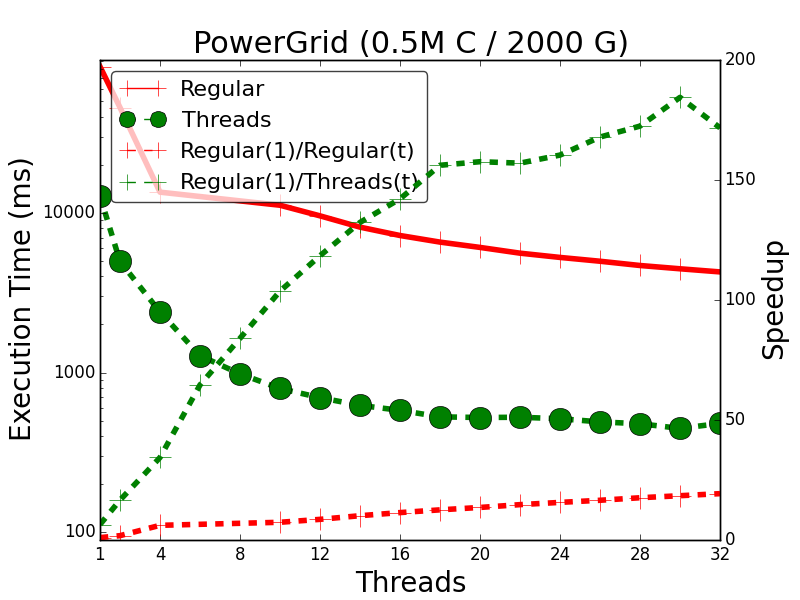
\includegraphics[width=\textwidth]{experiments/threads/cmp-powergrid-500000C2000G.png}
           \mycap{}
           \label{fig:threads:powergrid1}
        \end{subfigure}
        ~
        \begin{subfigure}[b]{\plotsize\textwidth}
           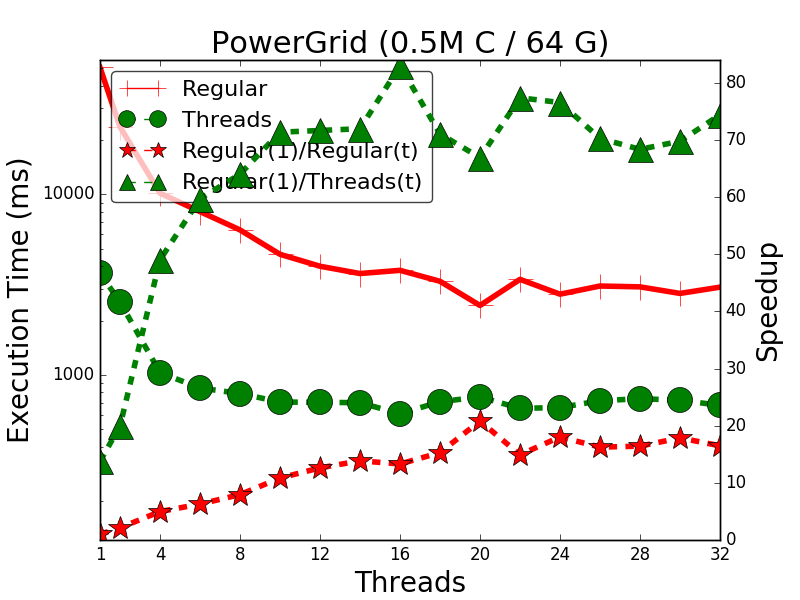
\includegraphics[width=\textwidth]{experiments/threads/cmp-powergrid-500000C64G.png}
           \mycap{}
           \label{fig:threads:powergrid2}
        \end{subfigure} \\
        \begin{subfigure}[b]{\plotsize\textwidth}
           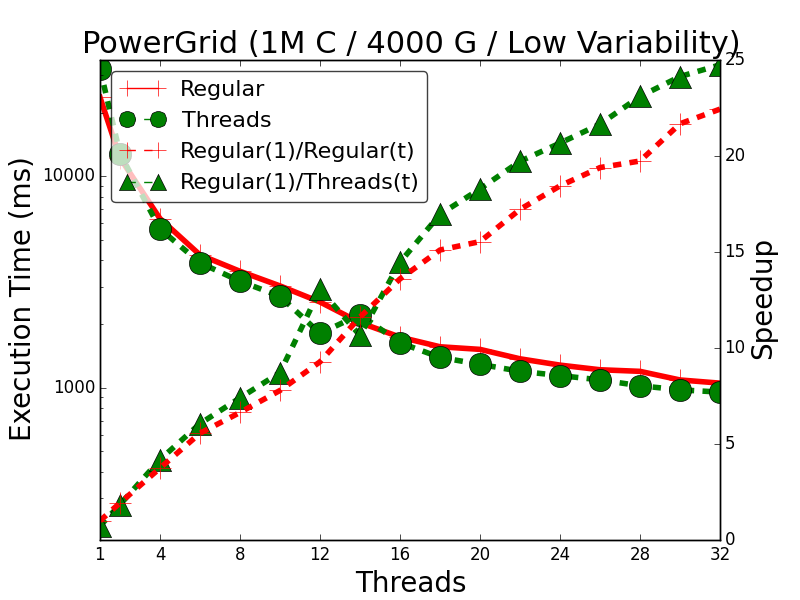
\includegraphics[width=\textwidth]{experiments/threads/cmp-powergrid-1M4000C-low.png}
           \mycap{}
           \label{fig:threads:powergrid3}
        \end{subfigure} ~
        \begin{subfigure}[b]{\plotsize\textwidth}
           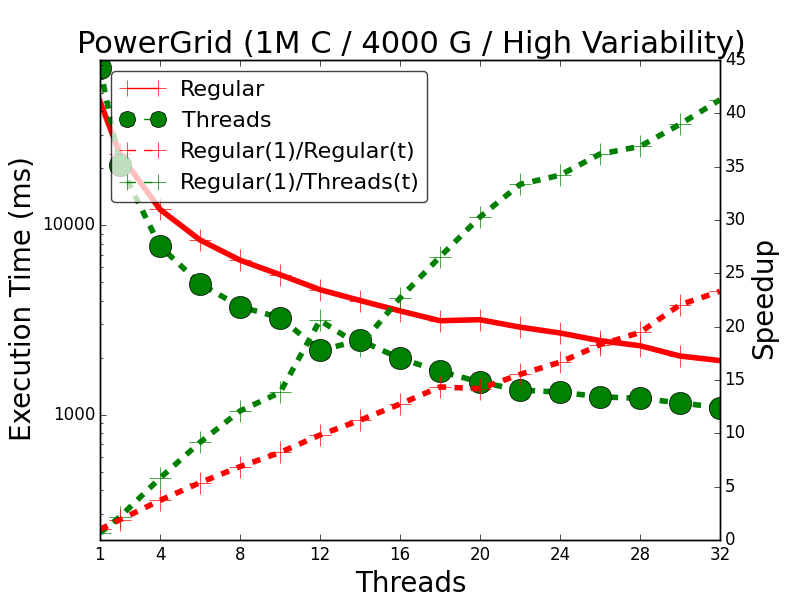
\includegraphics[width=\textwidth]{experiments/threads/cmp-powergrid-1M4000C-high.png}
           \mycap{}
           \label{fig:threads:powergrid4}
        \end{subfigure} \\
        \mycap{Measuring the performance of the PowerGrid program
        when using thread facts.}
        \label{fig:threads:results_powergrid}
\end{figure}

The second important observation relates to the last two datasets where we
experimented with a variable capacity for the generators. For the Low
Variability dataset, the consumers have identical capacities, while in the High
Variability dataset, generators have a more variable capacity, which should make
it harder for the algorithm to find a valid generator/consumer assignment.  Our
results show exactly that: the Low Variability shows a small difference between
the \textbf{Regular} and \textbf{Threads} version, while in the High Variability
dataset, the \textbf{Threads} version is much faster than the \textbf{Regular}
version. However, for the High Variability dataset, we were expecting a speedup
that was closer to the 0.5 M C / 2000 G dataset, since the number of generators
is much higher. Furthermore, if we compare the run times of the \textbf{Regular}
and \textbf{Threads} version when using 1 thread, we notice that the
\textbf{Threads} version is actually slower. As noted before, this may be due to
the fact that the LM rule for assigning generators to consumers needs to perform
a linear scan on the available generators to find a suitable generator which
then negatively impacts performance. This is a clear drawback of the logic
programming model that could potentially be solved by maintaining a sorted list
of \texttt{thread-capacity} facts.

In Table~\ref{table:threads:powergrid_stats}, we present several fact statistics
that compare the \textbf{Regular} version with the \textbf{Threads} version when
executing with multiple threads. The \textbf{\# Derived} column indicates the
number of derived facts, \textbf{\# Deleted} indicates the number of retracted
facts, while \textbf{\# Final} is the number of facts in the database after the
program terminates. The table results clearly show that using thread-based facts
results in a decrease in the number of generated facts, which is more
significant in the 0.5M C / 2000 G dataset (10-fold reduction). The table also
explains why this dataset performs much better than the 1M C / 4000 G High
Variability dataset, which only sees a 2-fold reduction in derived facts.

When comparing the number of facts derived when using a different number of
threads, the overall trend indicates that having more threads slightly increases
the number of derived facts. This is especially true for the 0.5 M C / 64 G
datasets, where twice as many facts are generated when using 32 threads when
compared to 1 thread.

\begin{table}[ht]
   \begin{center}
      \begin{tabular}{c | c || c c | c c | c c} \hline
	 \multirow{2}{*}{\textbf{Dataset}} & \multirow{2}{*}{\textbf{Threads}} & \multicolumn{2}{c|}{\textbf{\# Derived}} & \multicolumn{2}{c|}{\textbf{\# Deleted}} & \multicolumn{2}{c}{\textbf{\# Final}}\\
	 & & Regular & Threads & Regular & Threads & Regular & Threads\\ \hline \hline
\multirow{7}{*}{0.5M C / 2000 G}  & 1 &  49.7M & 4.2M &  48.2M & 2.5M &  2.5M & 2.5M \\
 & 2 &  48.5M & 4.4M &  47.7M & 2.5M &  2.5M & 2.5M \\
 & 4 &  49.4M & 4.1M &  47.9M & 2.6M &  2.5M & 2.5M \\
 & 8 &  49.4M & 4.10M &  47.9M & 2.5M &  2.5M & 2.5M \\
 & 16 &  50.8M & 4.1M &  49.3M & 2.6M &  2.5M & 2.5M \\
 & 24 &  49.8M & 4.2M &  48.3M & 2.7M &  2.5M & 2.5M \\
 & 32 &  49.3M & 4.6M &  47.8M & 3.1M &  2.5M & 2.5M \\
	\hline
\multirow{7}{*}{0.5M C / 64 G}  & 1 &  20.2M & 4.3M &  18.5M & 2.5M &  2.5M & 2.5M \\
 & 2 &  19.9M & 4.2M &  18.4M & 2.7M &  2.5M & 2.5M \\
 & 4 &  20.7M & 4.4M &  18.5M & 2.9M &  2.5M & 2.5M \\
 & 8 &  19.9M & 5.6M &  18.4M & 4.10M &  2.5M & 2.5M \\
 & 16 &  19.8M & 6.8M &  18.3M & 5.3M &  2.5M & 2.5M \\
 & 24 &  19.7M & 8.4M &  18.2M & 6.9M &  2.5M & 2.5M \\
 & 32 &  19.9M & 9.3M &  18.4M & 7.5M &  2.5M & 2.5M \\
	\hline
\multirow{7}{*}{\makecell{1M C / 4000 G \\Low Variability}}  & 1 &  9.4M & 7.5M &  6.4M & 4.5M &  5.1M & 5.1M \\
 & 2 &  9.4M & 7.5M &  6.4M & 4.5M &  5.1M & 5.1M \\
 & 4 &  9.4M & 7.5M &  6.4M & 4.5M &  5.1M & 5.1M \\
 & 8 &  9.4M & 7.6M &  6.4M & 4.6M &  5.1M & 5.1M \\
 & 16 &  9.4M & 7.5M &  6.4M & 4.5M &  5.1M & 5.1M \\
 & 24 &  9.4M & 7.6M &  6.3M & 4.6M &  5.1M & 5.1M \\
 & 32 &  9.3M & 7.5M &  6.3M & 4.5M &  5.1M & 5.1M \\
	\hline
\multirow{7}{*}{\makecell{1M C / 4000 G \\High Variability}}  & 1 &  16.4M & 8.8M &  13.4M & 5.8M &  5.1M & 5.1M \\
 & 2 &  16.5M & 8.8M &  13.5M & 5.8M &  5.1M & 5.1M \\
 & 4 &  16.5M & 8.8M &  13.4M & 5.8M &  5.1M & 5.1M \\
 & 8 &  16.5M & 8.9M &  13.5M & 5.9M &  5.1M & 5.1M \\
 & 16 &  16.5M & 8.8M &  13.5M & 5.8M &  5.1M & 5.1M \\
 & 24 &  16.5M & 9.3M &  13.5M & 6.2M &  5.1M & 5.1M \\
 & 32 &  16.5M & 9.6M &  13.5M & 6.5M &  5.1M & 5.1M \\
	\hline
\end{tabular}

   \end{center}

   \mycap{Measuring the reduction in derived facts when using thread-based
   facts.}
   \label{table:threads:powergrid_stats}
\end{table}

%\clearpage


\subsection{Splash Belief Propagation}
Approximation algorithms can obtain significant benefits from using customized
scheduling policies since they follow important statistical properties and thus
can trade correctness for faster convergence. An example of such algorithm is
the Loopy Belief Propagation (LBP)~\cite{Murphy99loopybelief}. LBP is an
approximate inference algorithm used in graphical models with cycles which
employs a sum-product message passing algorithm where nodes exchange messages
with their immediate neighbors and apply some computations to the messages
received.

\begin{figure}[h]
   \begin{center}
      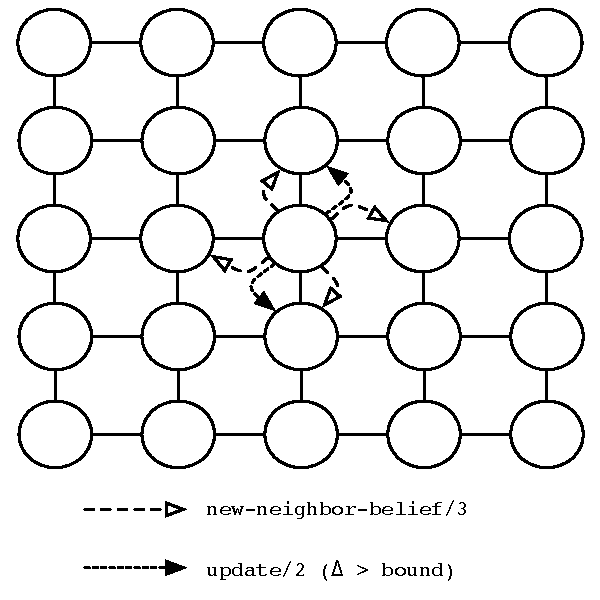
\includegraphics[width=0.3\textwidth]{figures/bp/bp.pdf}
   \end{center}

   \mycap{LBP communication patterns. \code{new-neighbor-belief} facts are
   sent to the neighborhood when the node's belief value is updated. If the new
   value sent to the neighbor differs significantly from the value sent before
   the current the round, then an \code{update} fact is also sent (to the node
   above and below in this case).}

\label{fig:coordination:bp}
\end{figure}

LBP is an algorithm that maps very well to the graph-based model of LM. The
original algorithm computes the belief of all nodes using several iterations
with synchronization between iterations. However, it is possible to avoid the
synchronization step, if we take advantage of the fact that LBP will converge
even when using an asynchronous approach. So, instead of computing the belief
iteratively, we keep track of all messages sent/received (and overwrite them
when we receive a new one) and recompute the belief asynchronously.
Figure~\ref{fig:coordination:bp} presents the communication patterns of the
program, while Fig.~\ref{code:coordination:bp} presents the LM code for the
asynchronous version of LBP.

\begin{figure}[ht]
\begin{Verbatim}[numbers=left, fontsize=\codesize, commandchars=\*\#\&]
type list float belief.*hfill// Type declaration.

type potential(node, belief).*hfill// Predicate declaration
type edge(node, node).
type linear neighbor-belief(node, node, belief).
type linear new-neighbor-belief(node, node, belief).
type linear sent-neighbor-belief(node, node, belief).
type linear check-residual(node, float, node).
type linear belief(node, belief).
type linear update-messages(node, belief).
type linear update(node).

neighbor-belief(A, B, Belief),*label#line:coord:bp_first1&*hfill// Rule 1: update neighbor belief value
new-neighbor-belief(A, B, NewBelief)
   -o neighbor-belief(A, B, NewBelief).*label#line:coord:bp_first2&

check-residual(A, Residual, B),*label#line:coord:bp_check1&*hfill// Rule 2: check residual
Residual > bound
   -o update(B).

check-residual(A, _, _) -o 1.*label#line:coord:bp_check2&*hfill// Rule 3: check residual

update-messages(A, NewBelief),*hfill// Rule 4: compute belief to be sent to a neighbor node*label#line:coord:bp_iterate1&
   -o {B, OldIn, OldOut, Cavity, Convolved, OutMessage, Residual |
         !edge(A, B),
         neighbor-belief(A, B, OldIn),
         sent-neighbor-belief(A, B, OldOut),
         Cavity = normalize(divide(NewBelief, OldIn)),
         Convolved = normalize(convolve(global-potential, Cavity)),
         OutMessage = damp(Convolved, OldOut, damping)
         Residual = residual(OutMessage, OldOut)
         -o check-residual(A, Residual, B),
            new-neighbor-belief(B, A, OutMessage),
            neighbor-belief(A, B, OldIn),
            sent-neighbor-belief(A, B, OutMessage)}.*label#line:coord:bp_iterate2&

*label#line:coord:bp_last1&
update(A), update(A) -o update(A).*label#line:coord:bp_update&*hfill// Rule 5: prune redundant update operations

update(A),*hfill// Rule 6: initiate update operation*label#line:coord:bp_update1&
!potential(A, Potential),
belief(A, MyBelief)
   -o [sum Potential => Belief; B, Belief |*label#line:coord:bp_agg1&
         neighbor-belief(A, B, Belief) -o
         neighbor-belief(A, B, Belief) ->
         Normalized = normalizestruct(Belief),
         update-messages(A, Normalized), belief(A, Normalized)].*label#line:coord:bp_last2&*label#line:coord:bp_update2&*label#line:coord:bp_agg2&
\end{Verbatim}

\mycap{LM code for the asynchronous version of the Loopy Belief Propagation
problem.}

\label{code:coordination:bp}
\end{figure}

\clearpage

Belief values are arrays of floats and are represented by \code{belief/2} facts.
The first rule (lines~\ref{line:coord:bp_first1}-\ref{line:coord:bp_first2})
updates a given neighbor belief whenever a new belief value is received. This is
the highest priority rule since we want to update the neighbor beliefs before
doing anything else. In order to store the belief values of the neighbor nodes,
we use \code{neighbor-belief/3} facts, where the second argument is the neighbor
address and the third argument is the belief value.

The last two rules (lines~\ref{line:coord:bp_last1}-\ref{line:coord:bp_last2})
update the belief value of a node. An \code{update} fact starts the process.
The first rule (line~\ref{line:coord:bp_update}) simply removes redundant
\code{update} facts and the second rule
(lines~\ref{line:coord:bp_update1}-\ref{line:coord:bp_update2}) performs the
belief update by aggregating all the neighbor belief values. The aggregate in
lines~\ref{line:coord:bp_agg1}-\ref{line:coord:bp_agg2} also derives copies of
the neighbors beliefs that need to be consumed in order to compute the belief
value that is going to be sent to the target neighbor. The aggregate uses a
custom accumulator that takes two arrays and adds the floating point numbers at
each index of the array.

The rule in lines~\ref{line:coord:bp_iterate1}-\ref{line:coord:bp_iterate2}
iterates through the neighbor belief values and sends new belief values by
performing the appropriate computations on the new belief value of the current
node and on the belief value sent previously. For each neighbor update, we also
check in lines~\ref{line:coord:bp_check1}-\ref{line:coord:bp_check2} if the
change in belief values is greater than \code{bound} (a program constant) and
then force the neighbor nodes to update their belief values by deriving
\code{update(B)}. This allows neighbor nodes to use updated neighbor values and
recompute their own belief values using more up-to-date information. The
computation of belief values will then start to converge to their true belief
values, independently of the node scheduling used.

However, if we prioritize nodes that receive new neighbor belief values with a
larger \code{Residual} then we may converge faster.
Figure~\ref{code:coordination:improved_bp} shows the fourth rule modified with a
\code{add-priority} fact, which increases the priority of neighbor nodes when
the source node has large changes in its belief value.

\begin{figure}[h!]
\begin{Verbatim}[numbers=left,commandchars=\\\{\},fontsize=\codesize]
update-messages(A, NewBelief),*hfill// Rule 4: compute belief to be sent to a neighbor node
   -o \{B, OldIn, OldOut, Cavity, Convolved, OutMessage, Residual |
         !edge(A, B),
         neighbor-belief(A, B, OldIn),
         sent-neighbor-belief(A, B, OldOut),
         Cavity = normalize(divide(NewBelief, OldIn)),
         Convolved = normalize(convolve(global-potential, Cavity)),
         OutMessage = damp(Convolved, OldOut, damping)
         Residual = residual(OutMessage, OldOut)
         -o check-residual(A, Residual, B),
            new-neighbor-belief(B, A, OutMessage),
            neighbor-belief(A, B, OldIn),
            \underline{add-priority(B, Residual)},
            sent-neighbor-belief(A, B, OutMessage)\}.
\end{Verbatim}
\mycap{Extending the LBP program with priorities.}
\label{code:coordination:improved_bp}
\end{figure}


The proposed asynchronous approach has shown to be an improvement over the
synchronous version because it leads to faster convergence time. An improved
evaluation strategy is the Splash Belief
Propagation~(SBP)~\cite{Gonzalez+al:aistats09paraml}, where belief values are
computed asynchronously by first building a tree and then updating the beliefs
of each node twice, first from the leaves to the root and then from the root to
the leaves These \emph{splash trees} are built by starting at a node whose
belief changed the most in the last update. The trees must be built iteratively
until convergence is achieved.

In an environment with $T$ threads, it is then possible to build $T$ splash
trees concurrently. First, we partition the nodes into $T$ regions and then
assign each region to a thread. A thread is then responsible for iteratively
building splash trees on that region until convergence is reached.
Fig.~\ref{fig:threads:splash_bp} shows a grid of nodes that has been partitioned
in two regions where splash trees will be built. To build a splash tree, a
thread starts from the highest priority node (the tree's root) from its region
and then performs a breadth-first search from that node to construct the rest of
the tree. The belief values are then computed in order.

\begin{figure}[ht]
   \begin{center}
      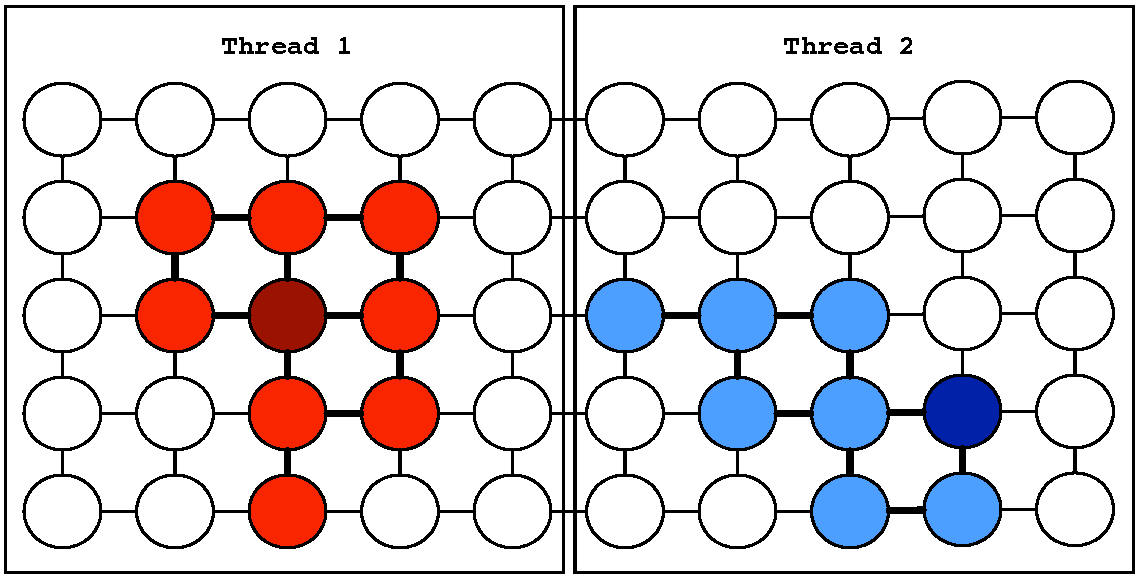
\includegraphics[width=0.7\linewidth]{figures/threads/splash_bp}
   \end{center}
   \caption{Creating splash trees using two threads. The graph is
      partitioned into two regions and each thread is able to build separate
   splash trees starting from the highest priority node.}
   \label{fig:threads:splash_bp}
\end{figure}

The LM implementation for SBP is shown in Fig.~\ref{code:threads:sbp}. First,
in lines \ref{line:threads:splash_part1}-\ref{line:threads:splash_part2}, we
partition the nodes into regions using \code{set-thread} and then we start the
creation of the first splash tree (line~\ref{line:threads:splash_first}) by
deriving \code{start-tree(T)}.  The remaining phases of the algorithm are
explained next.

\begin{figure}[!htb]
\begin{Verbatim}[numbers=left,commandchars=*\{\},fontsize=\codesize]
type list node tree.

type linear partitioning(thread, int). // Number of nodes to receive.
type linear start-tree(thread).
type linear new-tree(thread, tree, tree).
type linear expand-tree(thread, tree).
type linear first-phase(thread, tree, tree).
type linear second-phase(thread, tree).
type linear start(node).

start(A).
partitioning(T, @world / @threads). // Move @world/@threads nodes.

!coord(A, X, Y), start(A) // Moving this node.*label{line:threads:splash_part1}
   -o set-static(A), set-thread(A, grid(X, Y)).
just-moved(A), partitioning(T, Left) // Thread received another node.
   -o partitioning(T, Left - 1).
partitioning(T, 0) -o start-tree(T).*label{line:threads:splash_part2}*label{line:threads:splash_first}

start-tree(T),*label{line:threads:splash_building1} priority(A, P), P > 0.0 *hfill{} // Tree building
   -o priority(A, P), expand-tree(T, [A], []).*label{line:threads:splash_building2}
expand-tree(T, [A | All], Next)
   -o thread-id(A, Id),
      [collect => L ; | !edge(A, L), ~ L in All, ~ L in Next,*label{line:threads:splash_agg1} priority(L, P), P > 0.0,
         thread-id(L, Id2), Id1 = Id2 -o priority(L, P), thread-id(L, Id2) ->
         new-tree(T, [A | All],
            if len(All) + 1 >= maxnodes then [] else Next ++ L end)].*label{line:threads:splash_agg2}*label{line:threads:splash_next}

new-tree(T, [A | All], [])
   -o schedule-next(A), first-phase(T, reverse([A | All]), [A | All]).*label{line:threads:splash_first_phase}
new-tree(T, All, [B | Next])
   -o schedule-next(B), expand-tree(T, [B | All], Next).

first-phase(T, [A], [A]), running(T, A) *hfill{} // First phase
   -o running(T, A), update(A), remove-priority(A), start-tree(T).
first-phase(T, [A, B | Next], [A]), running(T, A)
   -o running(T, A), update(A), schedule-next(B), second-phase(T, [B | Next]).*label{line:threads:splash_first_update1}
first-phase(T, All, [A, B | Next]), running(T, A)
   -o running(T, A), update(A), schedule-next(B), first-phase(T, All, [B | Next]).*label{line:threads:splash_first_update2}

second-phase(T, [A]), running(T, A) *hfill{} // Second phase
   -o running(T, A), update(A), remove-priority(A), start-tree(T).*label{line:threads:splash_second_update1}
second-phase(T, [A, B | Next]), running(T, A)
   -o running(T, A), update(A), schedule-next(B), second-phase(T, [B | Next]).*label{line:threads:splash_second_update2}
\end{Verbatim}

   \caption{LM code for the Splash Belief Propagation program.}
  \label{code:threads:sbp}
\end{figure}

\begin{description}

   \item[Tree building:] Starts after the rule in lines
      \ref{line:threads:splash_building1}-\ref{line:threads:splash_building2} is
      derived. Since the thread always picks the highest priority node, we start
      by adding that node to the list that represents the tree. In lines
      \ref{line:threads:splash_agg1}-\ref{line:threads:splash_agg2}, we use an
      aggregate to gather all the neighbor nodes that have a positive priority
      (due to a new belief update) and are in the same thread. Nodes are
      collected into list \code{L} and appended to list \code{Next}
      (line~\ref{line:threads:splash_next}).

   \item[First phase:] When the number of nodes in the tree reaches a certain
      limit, a \code{first-phase} is generated to update the beliefs of all
      nodes in the tree (line~\ref{line:threads:splash_first_phase}). As the
      nodes are updated, starting from the leaves and ending at the root, an
      \code{update} fact is derived to update the belief values
      (lines~\ref{line:threads:splash_first_update1}
      and~\ref{line:threads:splash_first_update2}).

   \item[Second phase:] Performs the computation of beliefs from the root to the
      leaves and the belief values are updated a second time
      (lines~\ref{line:threads:splash_second_update1}
      and~\ref{line:threads:splash_second_update2}).

\end{description}

SBP is also implemented in GraphLab~\cite{GraphLab2010}, a C++ framework for
writing machine learning algorithms. GraphLab provides the splash scheduler as
part of its framework. We measured the behavior of LBP and SBP for both LM and
GraphLab. Fig.~XXX shows that both systems have very similar behavior when using
a variable number of threads, but for higher number of threads and, in
particular, for more than 15 threads, LM shows better speedups than GraphLab. In
terms of running times, LM is, on average, 1.4 times slower than GraphLab,
although LM program code is more concise.


\section{Modeling the Operational Semantics in Linear Logic}
\subsection{Scheduling}

\section{Experimental Evaluation}

\section{Chapter Summary}

In this chapter, we have extended the LM language with a declarative mechanism
for reasoning about the underlying parallel architecture. LM programs can be
first written in a data-driven fashion and then optimized by reasoning about the
state of threads, enabling the move from implicit parallelism to explicit
parallelism. We have presented four programs that showcase the potential of the
new mechanism and several experimental results that validate our approach.

